\documentclass[12pt]{article}
\usepackage[italian]{babel}
\usepackage{geometry}
\usepackage{amsmath}
\usepackage{amssymb}
\usepackage{graphicx}
\usepackage{ulem}
\usepackage{tikz}

\usetikzlibrary{er, positioning}
\usetikzlibrary{arrows}

\geometry{margin=2cm}
\let\olditemize\itemize
\renewcommand\itemize{\olditemize\setlength\itemsep{0em}}

\tikzset {multi attribute/.style={attribute,double distance=1.5pt}}
\tikzset {derived attribute/.style={attribute,dashed}}
\tikzset {total/.style={double distance=1.5pt}}
\tikzset {every entity/.style={ draw=orange,fill=orange!20}}
\tikzset {every attribute/.style={draw=purple,fill=purple!20}}
\tikzset {every relationship/.style={draw=green,fill=green!20}}
\newcommand {\key}[1]{\underline{#1}}

\title{Schema ER (Parte 3)}
\author{Lorenzo Vaccarecci}
\date{14 Marzo 2024}

\graphicspath{{../Immagini/}}

\begin{document}
\maketitle
\section{Sottoinsieme}
\begin{center}
    \begin{tikzpicture}[auto, node distance=2cm]
        \node[entity](e){E};
        \node[entity](e')[below of=e]{E'};
        \path[<-] (e) edge node {} (e');
    \end{tikzpicture}
\end{center}
\section{Esercizio Wooclap}
\begin{center}
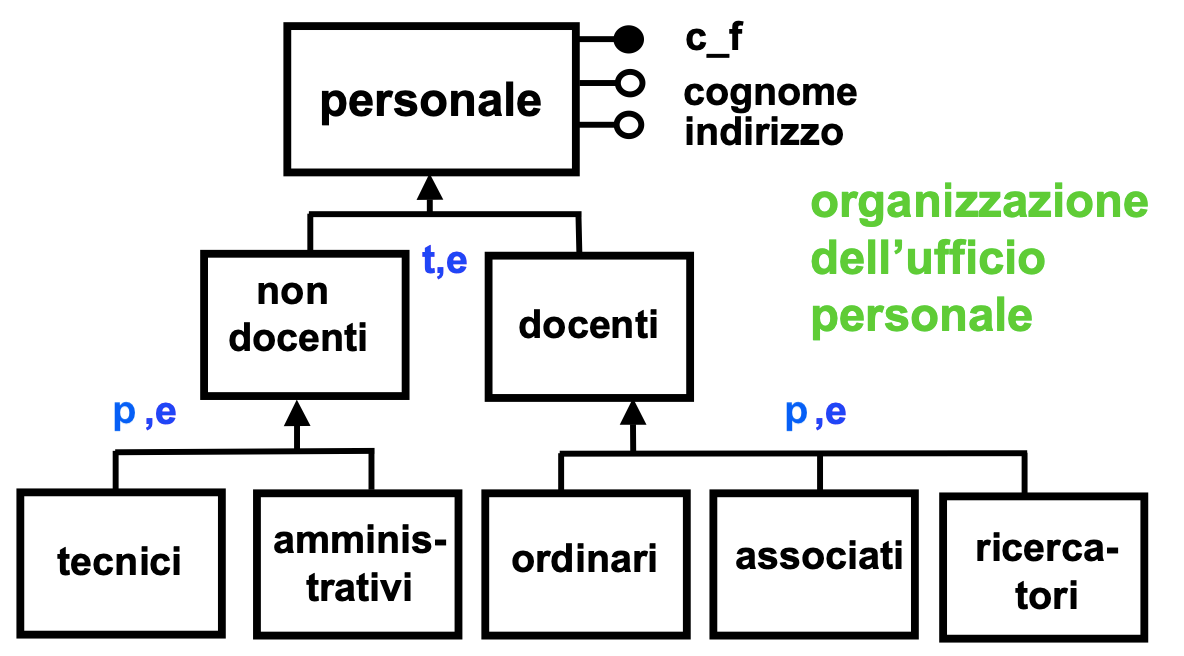
\includegraphics[width=\textwidth]{modelloer1.png}
\end{center}
\textit{In riferimento alla gerarchia in figura, quali affermazioni sono vere?}\\
\begin{description}
    \item[$\boxtimes$] ogni unità di personale è certamente docente oppure non docente
    \item[$\boxtimes$] nessuna unità di personale può essere contemporaneamente docente e non docente
    \item[$\boxtimes$] ogni docente è certamente un prof ordinario, oppure un prof associato oppure un ricercatore
    \item[$\boxtimes$] nessun docente può essere contemporaneamente prof ordinario e ricercatore 
\end{description}
\end{document}